\chapter{Related work} \label{chap3}

\section{Bibliographical research methodology} \label{3biblio_research}

To define the state-of-the-art for ECG classification and Federated learning I performed a reduced Systematic Review. The latter is defined as \cite{systematic_review} a 'process of critically evaluating, summarizing, and seeking to reconcile the evidence.' In other words, it is a complete evaluation of literature that differs from a traditional review in that it is undertaken in a methodical (or systematic) manner, following a pre-specified process to avoid bias, with the goal of synthesizing the information gathered. 

Then the first step to perform the systematic review (SR or bibliographical research) was to decide the reference and citation databases to use. In the table \ref{table:dbs_sr} are written the academic search engines used to retrieve the related documents.

\begin{table}[H]
\begin{center}
% \resizebox{\textwidth}{!}{
\begin{tabular}{||p{0.2\linewidth} || p{0.55\linewidth} | p{0.15\linewidth}||}
 \hline
\textbf{Search Engine} & \textbf{Definition} & \textbf{Link} \\ [0.4ex] 
 \hline\hline
Google Scholar & A free web search engine that indexes the full text or metadata of scholarly literature from a variety of publishers and fields. & \href{https://scholar.google.com/}{Link to GS} \\
\hline
PubMed.gov & Contains almost 34 million citations from MEDLINE, life science journals, and online books for biomedical literature. & \href{https://pubmed.ncbi.nlm.nih.gov/}{Link to PM} \\
\hline
IEEEXplore & A research database that allows users to access journal articles, conference proceedings, technical standards, etc. in computer science, electrical engineering, and electronics. & \href{https://ieeexplore.ieee.org/Xplore/home.jsp}{Link to IE} \\
\hline
Scopus & Has a huge collection of Physical Sciences and Engineering papers, from foundational science to novel and unique research, and spanning many disciplines both theoretical and applied. & \href{https://www.sciencedirect.com/}{Link to SCs} \\
\hline
Web Of Science & It is the most reliable publisher-independent worldwide citation database in the world. & \href{https://clarivate.com/webofsciencegroup/solutions/web-of-science/}{Link to WoS} \\
\hline
Papers with code & Their goal is to provide a free and open library that includes Machine Learning articles, code, datasets, methodologies, and evaluation tables. & \href{https://paperswithcode.com/}{Link to PwC} \\
\hline\hline
\end{tabular}
% }
\end{center}
\caption{Databases (search engines) used to find documents}
\label{table:dbs_sr}
\end{table}

From the previous graph we can see that most of the papers where published after 2017. That is because the concept of Federated Learning was introduced by Google in that year. Nevertheless, ECG classification is a topics that has been worked back in the 2000s. Moreover, the search engine that produced the highest number of resources was Web Of Science. 

Continuing with the analysis of figure \ref{fig:prisma_flow}, during the Screening phase I removed the duplicated documents keeping 1,600. After a fast screening (only title), I ended up with 317 possibly useful resources. During the eligibility phase, I screened the latter (title and abstract), ending up with 209 promising papers. Next, after assessing the keywords (given in the queries), I  reached 176 papers that were not read but were used to extract those keywords. On the other hand, I read 33 documents , from where 2 where not useful. That's the process how I found the 31 most useful papers after the research.

\section{ECG classification} \label{3state_art_ECG}

After reading the aforementioned documents, I gather some relevant highlights regarding the classification of ECG signals. Along the following paragraphs I summarize the most important findings at each topic.

\subsection{Techniques to handle imbalanced data}

In general, imbalanced data describes datasets in which the target class has an unequal distribution of observations. For example, when one class label has a large number of observations while the other has a small number.The authors who have dealt with this topic followed different paths to tackle this issue. Authors from \cite{imbalance_data1} introduced a \textit{Balanced Accuracy (BACC)} and the \textit{Matthew’s Correlation Coefficient (MCC)} to correct the fact that the classes don't share a similar distribution. In the article \cite{imbalance_data2} it was introduced the \textit{Generative Adversarial Network (GAN)} which deals with imbalanced data by generating and using additional fake data for detection purpose. In addition, \cite{imbalance_data3} used the \textit{Synthetic Minority Oversampling Technique (SMOTE)}, which is an oversampling technique. 

Other approaches also include the so-called \textit{Ratio Loss} (\cite{imbalance_data4}) where the global node estimates the composition data each round. When detecting an imbalanced composition continuously, the system acknowledges the class imbalance and load the Ratio Loss. One final possibility is the \textit{Recall of data} in which one randomly augment the lower class and in each training epoch change the selected individuals. Then, there are enough possibilities tried in the literature, each of of them with their pros and cons that can be verified further.



\subsection{Methods for ECG classification} \label{methods_ECG_class}

Along the literature I could find that a huge amount of diverse techniques have been applied when classifying ECG' arrhythmias. As an example \cite{ecg_methods1}, \cite{ecg_methods2}, and \cite{ecg_methods3} focused their efforts on Using Deep Neural Networks (Artificial Neural Networks and Multi-layer Perceptron) to get a model that predicts the abnormality given the ECG signal. In comparison, the author of \cite{ecg_methods4} combined in his paper the use of Naïve Bayes, Adaboost, Random Forest and Support Vector Machines to get the best classifier for his paper. Finally, \cite{ecg_methods5}, \cite{ecg_methods6} and \cite{ecg_methods7} employed in their research some Convolutional Neural Network approaches. Among them the highlighted Squeezenet, Attention mechanism and Resnet as the champion methods to deal with the ECG detection.

 \begin{figure}[H]
\centering
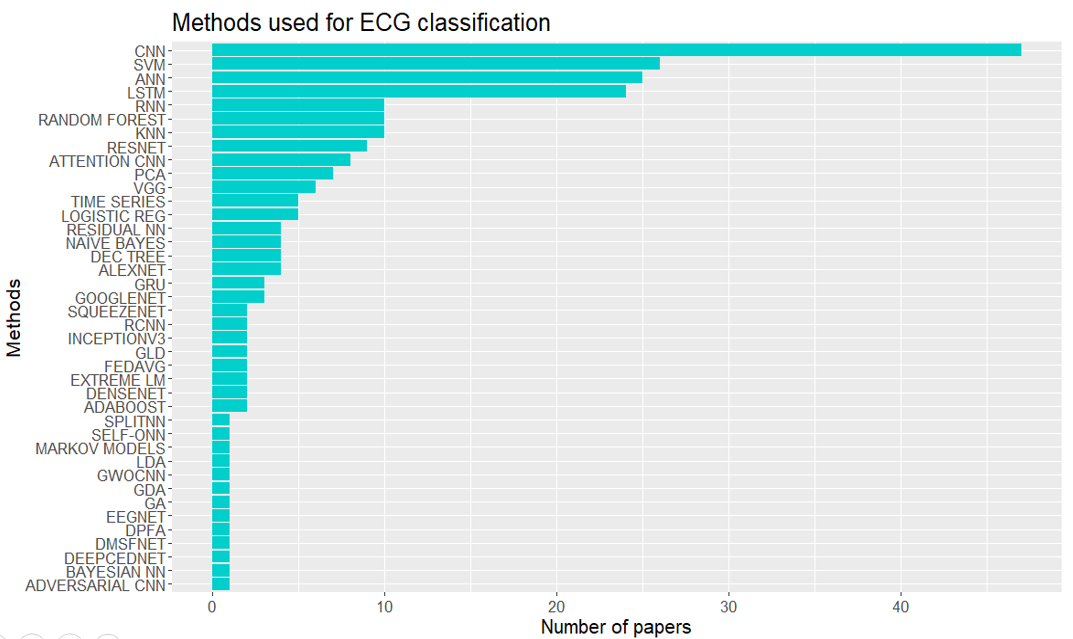
\includegraphics[scale=0.48]{img/classif_methods.PNG}
\caption{Most used classification methods for ECG}
\label{fig:classif_methods}
\end{figure}

As depicted in figure \ref{fig:classif_methods}, the most used technique is the Convolutional Neural Network (CNN). That one includes also some self-made Deep Neural Networks (DNN). On the second place we find Support Vector Machines (SVM) and Artificial Neural Networks (ANN). An very close to them most of the author also used Long-Short Term Memory (LSTM) algorithms. On the opposite, a few papers contributed with techniques like GWOCNN, DFPA, DEEPCETNET, etc, which are also CNN but that have specific alterations adapted to by the papers' authors.

\subsection{Metrics for ECG classification}\label{chap3metrics}

With respect to ECG arrhythmia classification, there are plenty of measurements employed in the literature. In figure \ref{fig:metrics_ECG} I show the most relevant metrics used in this aim, gathered from the available articles and papers shown in chapter \ref{3biblio_research}. 

 \begin{figure}[H]
\centering
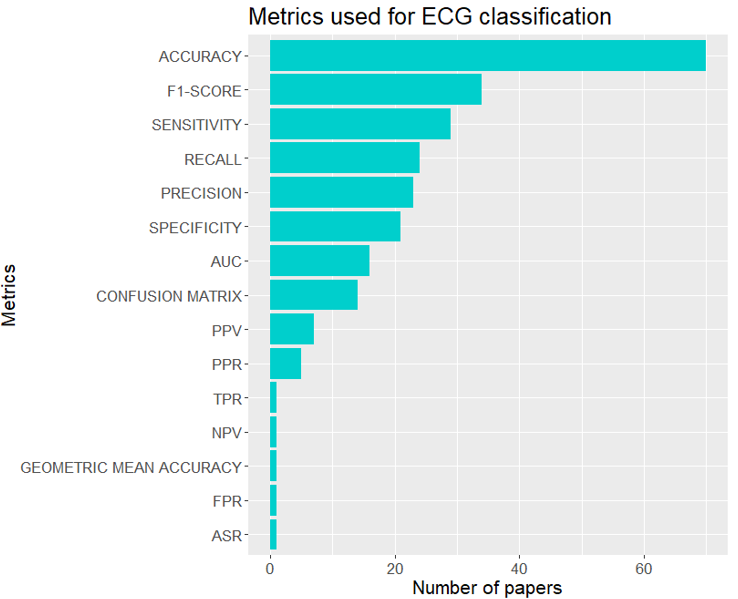
\includegraphics[scale=0.48]{img/metrics_ECG.PNG}
\caption{Most used metrics for ECG}
\label{fig:metrics_ECG}
\end{figure}

From the previous chart it is evident that the most used measure is the \textbf{Accuracy}. In the second place, the \textit{F1-Score} is often used. It is important to clarify that the latter is preferred when dealing with unbalanced data, since it take into account both \textit{Recall} and \textit{Precision} for its calculation. Some papers that consider the 4 mentioned measures at the same time can be found in \cite{metrics_ecg1}, 
\cite{metrics_ecg2} and \cite{metrics_ecg3}.



\subsection{Methods to handle NON-IID data} \label{non_iid_handling}

Along the literature, the researches performed have been focused on tackling the Non Independent Nor Identical distributed (Non-IID) problem that make the models in FL under-perform. In the following part I present a summary of the most relevant techniques used to deal with the mentioned issue.

\textbf{Over/under-sampling}: This is one of the most common techniques used to balance the data. It consist of randomly creating (or removing) data to equate distributions. The simplest way to do it is called Random Oversampling (ROS). The latter is the process of randomly picking and replacing instances from the minority class in the training dataset. There are other techniques like SMOTE \cite{metrics_ecg1}. SMOTE is a data augmentation algorithm that creates synthetic data points depending on the original data points. The technique can be thought of as a more advanced variant of oversampling or as a specific data augmentation process. SMOTE has the advantage of not creating duplicate data points, but rather synthetic data points that are somewhat different from the original data points \cite{imbalance_data3}.

\begin{figure}[H]
\centering
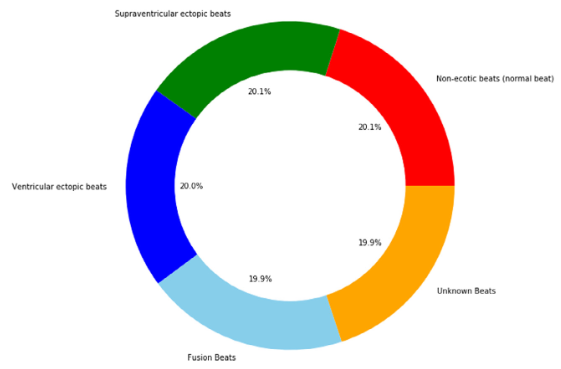
\includegraphics[scale=0.6]{img/metrics_ecg1_ROS.PNG}
\caption{The distribution of the up-sampled (re-balanced) dataset. \cite{metrics_ecg1}}
\label{fig:metrics_ecg1_ROS}
\end{figure}
